% Configuration space — the clustering x representation plane.
%
% ── WHAT THIS FIGURE IS FOR ───────────────────────────────────────────────
% The manuscript's central claim about the software is one sentence: "Common
% time series aggregation methods, such as k-means and k-medoids, strictly
% couple clustering and representation. ETHOS.TSAM allows users to combine
% clustering and representation methods flexibly." That claim has no figure.
% This is it: the plane is every valid configuration, the shaded cells are the
% six pairings the classical methods hard-wire, and the difference between the
% two is the contribution.
%
% The shaded cells are NOT hand-picked. They are exactly the entries of
% DEFAULT_REPRESENTATION in src/tsam/config.py:33-40 — the representation each
% clustering method falls back to when ClusterConfig.representation is unset:
%     averaging -> mean          kmeans   -> mean
%     kmedoids  -> medoid        kmaxoids -> maxoid
%     hierarchical -> medoid     contiguous -> medoid
% Note the pattern is NOT a diagonal: three of the six methods collapse onto
% `medoid`, which is itself part of the point — the classical coupling is
% coarser than the method list suggests.
%
% ── PRINT TARGET ──────────────────────────────────────────────────────────
% US Letter, 1 inch margins, text column 165.1 x 228.6 mm, figures placed at
% full text width. ASPECT h/w <= 1.24, and WIDTH <= ~165 mm so Word's scale
% factor stays 1.00 and \scriptsize prints at 8 pt.
%
% ── LAYOUT GRID (millimetres, y negative downwards) ───────────────────────
%   row labels   right-aligned, ending at x = 37
%   columns      centres 50 70 90 110 130 150, cell width 20
%   rows         centres -26 -39 -52 -65 -78 -91, cell height 13
%   grid extent  x 40 .. 160,  y -19.5 .. -97.5
%   column labels rotated 45 deg, anchored south west at (centre, -18).
%     A 12-character \scriptsize label rotated 45 deg reaches about 13.5 mm
%     right and 13.5 mm up, so the last column (centre 150) ends near x 163.5
%     and the tallest label tops out near y -4. Both are inside the budget;
%     re-check this if a longer method name is ever added.
%   axis title y -99.5, band heading y -109, chips y -122 (9 mm tall, so
%   -117.5 .. -126.5), key y -132. The heading is held clear of BOTH the
%   x-axis title above it and the chips below it; at -104 it collided with
%   the axis title, at -115 the chips collided with the heading.
%
% ── TRAPS RE-CHECKED HERE (see the project notes) ─────────────────────────
%   * every node carries an explicit `text width` to wrap against, and
%     `inner sep=0` on the full-width prose blocks, or they set the width.
%   * `distribution\_minmax` cannot break at `\_`, so it is broken by hand.
%   * \textperiodcentered{} and ---, never literal UTF-8 middots or em dashes.
%
% Regenerate:
%   tectonic configuration_space.tex
%   pdftocairo -svg configuration_space.pdf configuration_space.svg

\documentclass[10pt,border=1mm]{standalone}
\usepackage[T1]{fontenc}
\usepackage{lmodern}
\usepackage{tikz}
\usetikzlibrary{positioning,arrows.meta,fit,backgrounds,calc,shapes.geometric}

\definecolor{fzjblue}{HTML}{023D6B}
\definecolor{fzjdark}{HTML}{012845}
\definecolor{tintblue}{HTML}{DCE9F2}
\definecolor{amber}{HTML}{A8681A}
\definecolor{ambertint}{HTML}{FBF1E4}
\definecolor{greytext}{HTML}{3F4A55}
\definecolor{extline}{HTML}{8A94A0}

\newcommand{\ax}{\footnotesize\bfseries\color{fzjblue}}

\begin{document}
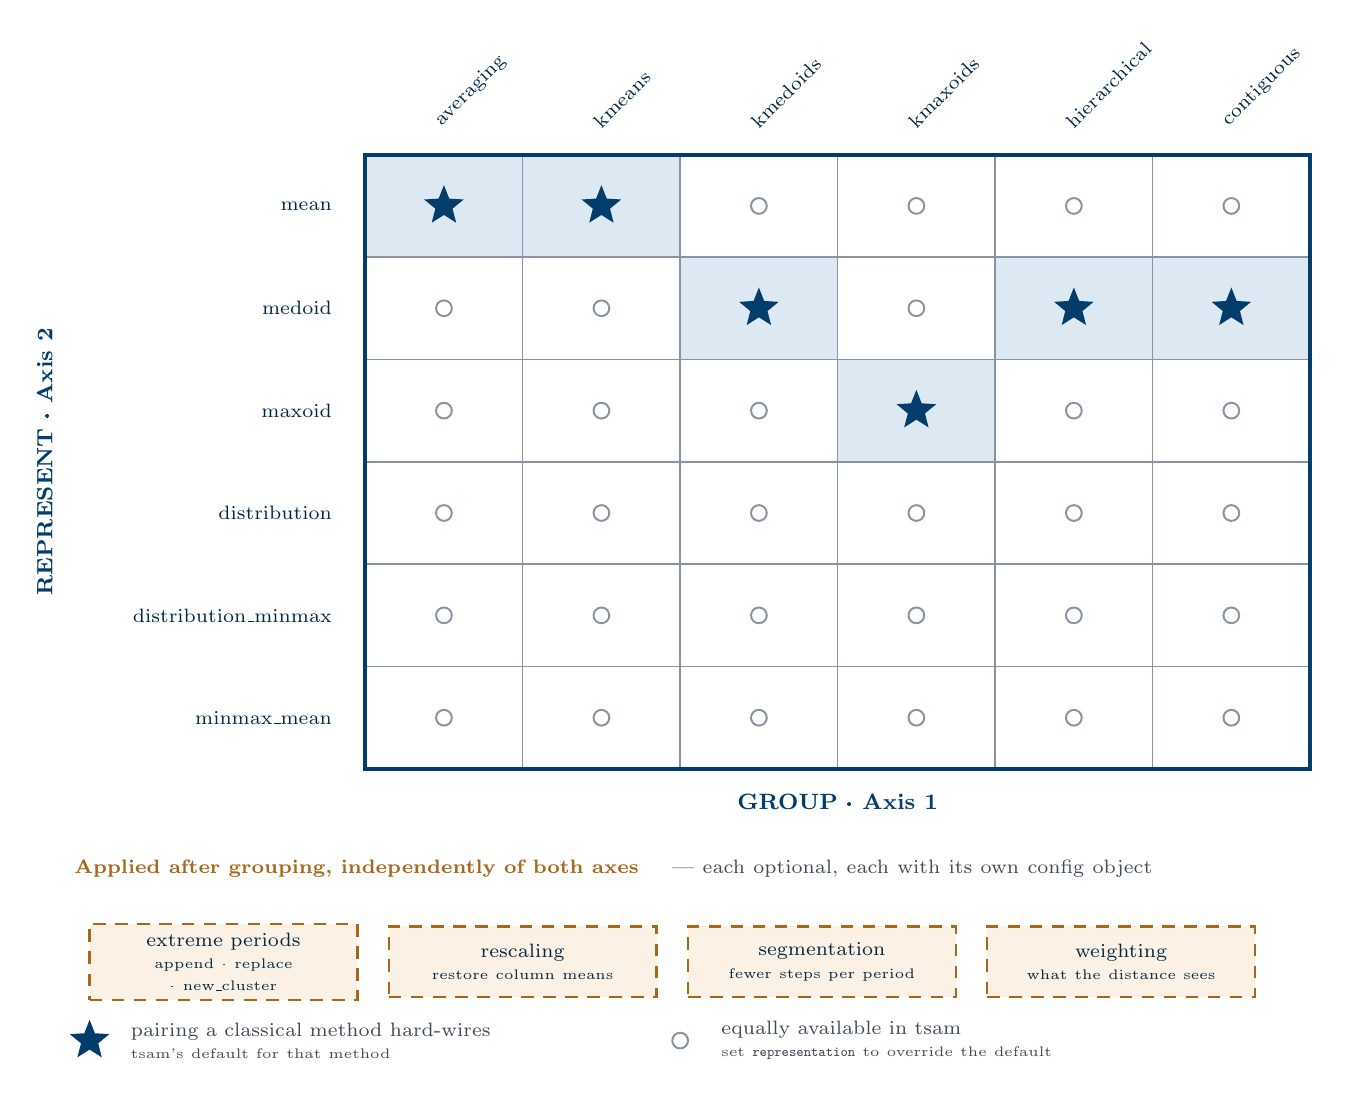
\begin{tikzpicture}[
  x=1mm, y=1mm,
  gridline/.style={draw=extline, line width=0.2mm},
  frame/.style={draw=fzjblue, line width=0.5mm},
  % a cell only tsam offers
  open/.style={circle, draw=extline, line width=0.25mm, fill=white,
               minimum size=2mm, inner sep=0},
  % a cell the classical method hard-wires
  fixed/.style={star, star points=5, star point ratio=2.3,
                draw=fzjblue, line width=0.25mm, fill=fzjblue,
                minimum size=4.6mm, inner sep=0},
  rlbl/.style={anchor=east, font=\scriptsize, text=fzjdark,
               align=right, text width=32mm},
  clbl/.style={anchor=south west, rotate=45, font=\scriptsize, text=fzjdark},
  % 9 mm, not 7: the extreme-periods chip needs three lines, and a TikZ node
  % clips nothing — at 7 mm its last line simply hung below the border.
  chip/.style={draw=amber, line width=0.3mm, dash pattern=on 1.6mm off 1.2mm,
               fill=ambertint, text=fzjdark, minimum width=34mm,
               minimum height=9mm, text width=31mm, align=center,
               font=\scriptsize},
  lgd/.style={font=\scriptsize, text=greytext, anchor=west}
]
\hyphenpenalty=10000 \exhyphenpenalty=10000

% ══ shaded cells: the six DEFAULT_REPRESENTATION pairings ══════════════════
% drawn first, on the background, so the grid rules stay visible on top
\foreach \cx/\cy in {50/-26, 70/-26, 90/-39, 110/-52, 130/-39, 150/-39}{
  \fill[tintblue] (\cx-10,\cy-6.5) rectangle (\cx+10,\cy+6.5);
}

% ══ grid ═══════════════════════════════════════════════════════════════════
\foreach \gx in {40,60,80,100,120,140,160}{
  \draw[gridline] (\gx,-19.5) -- (\gx,-97.5);
}
\foreach \gy in {-19.5,-32.5,-45.5,-58.5,-71.5,-84.5,-97.5}{
  \draw[gridline] (40,\gy) -- (160,\gy);
}
\draw[frame] (40,-19.5) rectangle (160,-97.5);

% ══ axis titles ════════════════════════════════════════════════════════════
% The vertical one is rotated as a whole node, so it needs no text width.
\node[rotate=90, anchor=south, font=\footnotesize\bfseries, text=fzjblue]
  at (1.5,-58.5) {REPRESENT \textperiodcentered{} Axis 2};
\node[anchor=north, font=\footnotesize\bfseries, text=fzjblue, text width=120mm,
      align=center] at (100,-99.5) {GROUP \textperiodcentered{} Axis 1};

% ══ row labels — values of ClusterConfig / SegmentConfig .representation ═══
\node[rlbl] at (37,-26) {mean};
\node[rlbl] at (37,-39) {medoid};
\node[rlbl] at (37,-52) {maxoid};
\node[rlbl] at (37,-65) {distribution};
\node[rlbl] at (37,-78) {distribution\_minmax};
\node[rlbl] at (37,-91) {minmax\_mean};

% ══ column labels — values of ClusterConfig.method ════════════════════════
\node[clbl] at ( 50,-18) {averaging};
\node[clbl] at ( 70,-18) {kmeans};
\node[clbl] at ( 90,-18) {kmedoids};
\node[clbl] at (110,-18) {kmaxoids};
\node[clbl] at (130,-18) {hierarchical};
\node[clbl] at (150,-18) {contiguous};

% ══ cells ══════════════════════════════════════════════════════════════════
\foreach \cx in {50,70,90,110,130,150}{
  \foreach \cy in {-26,-39,-52,-65,-78,-91}{
    \node[open] at (\cx,\cy) {};
  }
}
% the six fixed pairings, drawn over the open markers they replace
\foreach \cx/\cy in {50/-26, 70/-26, 90/-39, 110/-52, 130/-39, 150/-39}{
  \node[fixed] at (\cx,\cy) {};
}

% ══ the modifier band — everything that is NOT on either axis ═════════════
% Kept to ONE line: at two lines this heading reached y -112 and ran into the
% chips below it.
\node[anchor=north west, font=\scriptsize\bfseries, text=amber, text width=155mm,
      align=left, inner sep=0] at (3,-109)
  {Applied after grouping, independently of both axes
   \quad{\normalfont\color{greytext}--- each optional, each with its own
   config object}};
\node[chip] at ( 22,-122) {extreme periods\\{\tiny append \textperiodcentered{}
                            replace \textperiodcentered{} new\_cluster}};
\node[chip] at ( 60,-122) {rescaling\\{\tiny restore column means}};
\node[chip] at ( 98,-122) {segmentation\\{\tiny fewer steps per period}};
\node[chip] at (136,-122) {weighting\\{\tiny what the distance sees}};

% ══ key ════════════════════════════════════════════════════════════════════
\node[fixed] at (5,-132) {};
\node[lgd, text width=62mm] at (9,-132)
  {pairing a classical method hard-wires\\{\tiny tsam's default for that method}};
\node[open] at (80,-132) {};
\node[lgd, text width=70mm] at (84,-132)
  {equally available in tsam\\{\tiny set \texttt{representation} to override the default}};

\end{tikzpicture}
\end{document}
